\begin{figure*}
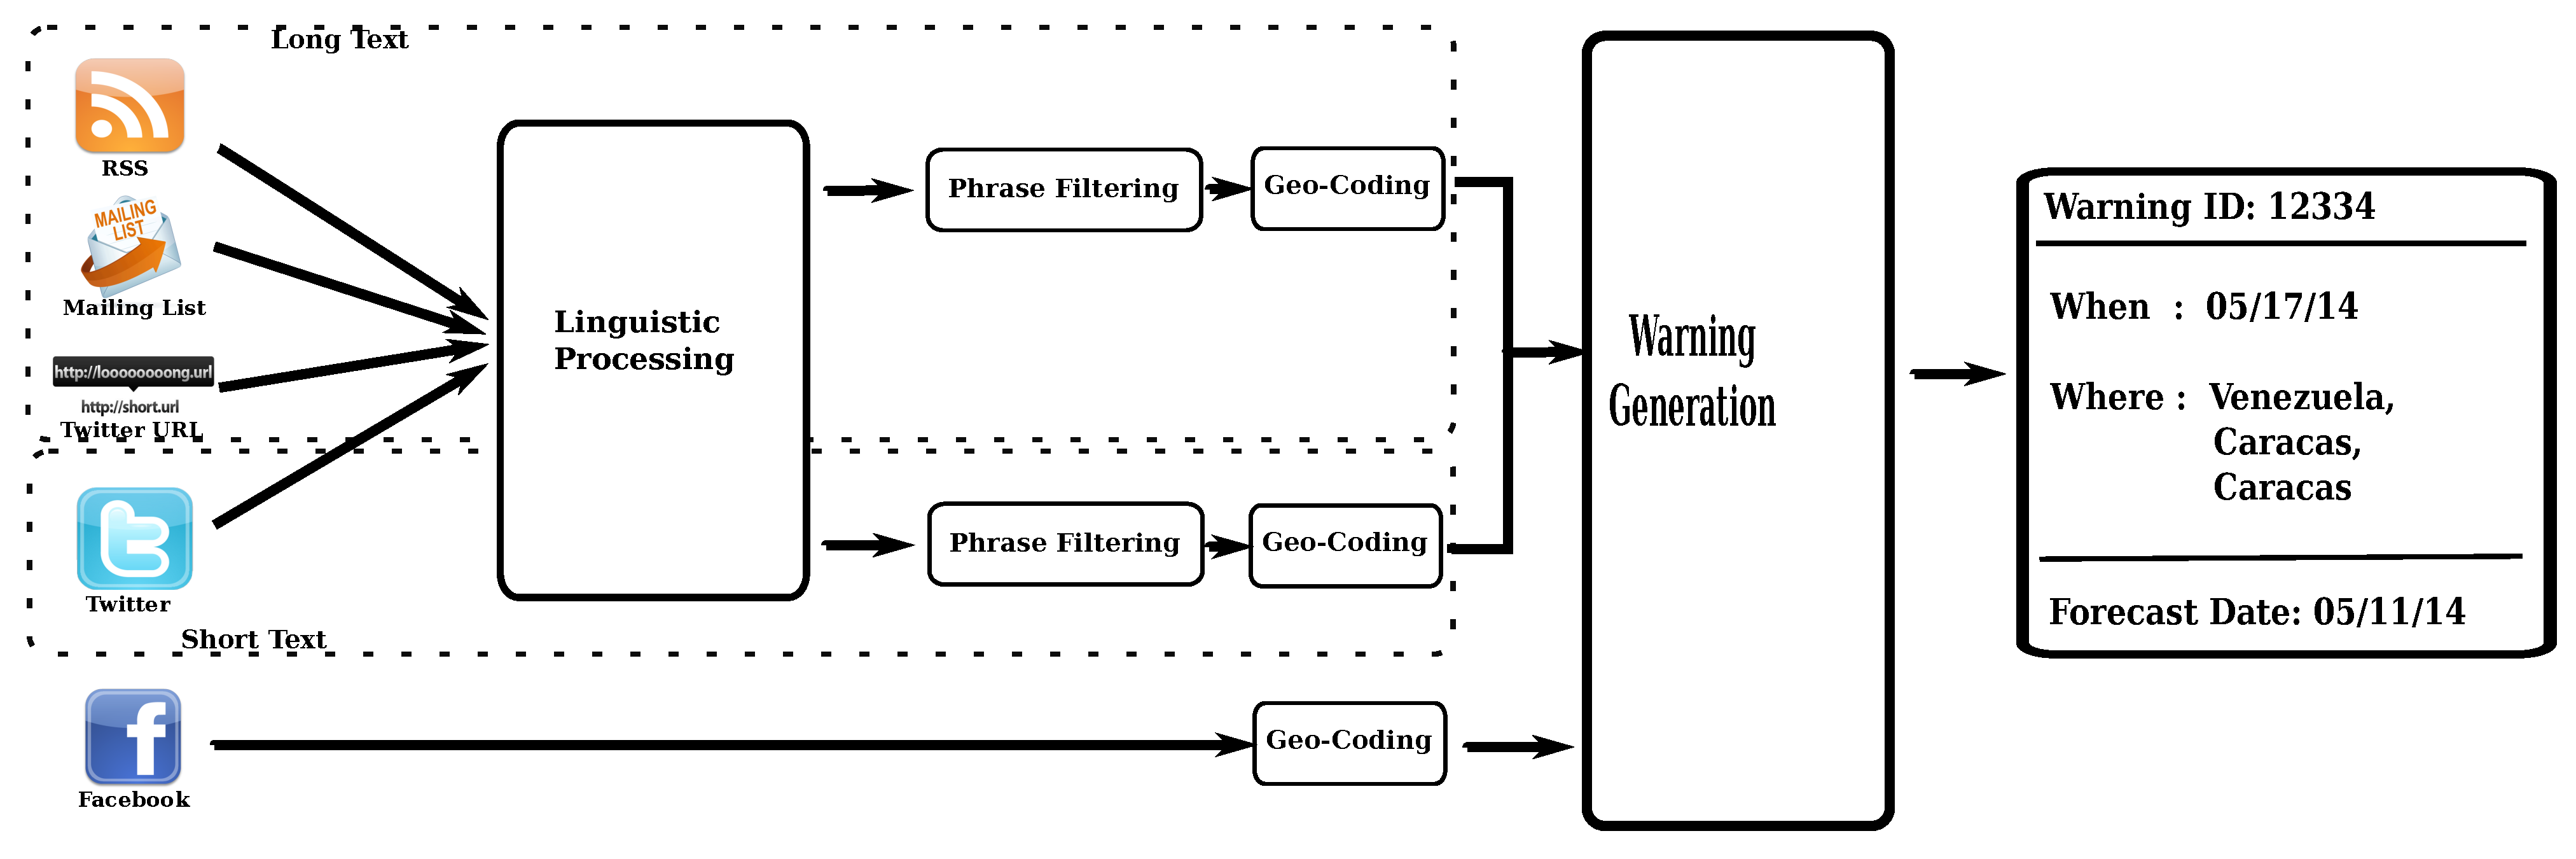
\includegraphics[width=\textwidth]{pipeline}
\vspace{-2em}
\caption{Schematic of the planned protest detector that ingests five
different types of data sources.}
\label{flowchart}
\end{figure*}
The general approach we adopt is to identify open-source documents
that appear to indicate civil unrest event planning, to extract
relevant information from identified documents and use that as the
basis for a structured warning about the planned event (see Fig.~\ref{flowchart}).
We ingest a
wide array of textual documents, including RSS feeds (news and blogs),
mailing lists, URLs referenced in tweets, the contents of the tweets themselves,
and Facebook event pages.
All harvested documents are subjected to linguistic analysis; candidate
documents are identified using a list of (learnt) phrases associated with
protest event planning; date and location information is extracted from the
text and reasoned about to generate a warning. Location information is standardized
to conform to a standard (in our case, we use the World Gazeteer).
Each of these processing
steps (see Fig.~\ref{flowchart}) is outlined next.

\subsection{Linguistic Preprocessing}
All textual input (e.g., tweets, news articles, blog postings) is
subjected to shallow linguistic processing prior to analysis.  This
involves identifying the language of the document, distinguishing the
the words (tokenization), normalizing words for inflection
(lemmatization), and identifying expressions referring to people,
places, dates and other entities and classifying them (named entity extraction). 
Since our region of interest is Latin America, the collection of text
harvested is inherently multilingual, with Spanish, Portugese, and English as
the dominating languages;
we use Basis Technology's Rosette Linguistics Platform (RLP) suite of multilingual commercial tools (\url{http://www.basistech.com/text-analytics/rosette/})for this stage.
The output of linguistic preprocessing serves as input to subsequent deeper analysis in which 
date expressions are normalized and the geographic focus of the text identified.

Date processing is particularly crucial to the identification of
future oriented statements. We use the TIMEN~\cite{LlorensDGS12} date
normalization package to normalize and deindex expressions referring
to days in English, Spanish and Portuguese. This system makes use of
meta-data such as the day of publication, and other information about
the linguistic context of the date expression to determine for each
date expression, what day (or week, month or year) it refers to.  For
example in a tweet produced on June 10, 2014, the occurrence of the
term {\em Friday} used in a future-tense sentence {\em We'll get
  together on Friday} will be interpreted as July 13, 2014.  Each
expression identified as a date by the RLP preprocessor is normalized
in this way.

\subsection{Phrase filtering}
In order to identify relevant documents, input documents are filtered on a set of key phrases, i.e.,
the text of the document is searched for the presence of one or
more key phrases in a list of phrases which are indicative of an article's focus being
a planned civil unrest event.  
The list of key phrases indicating civil unrest planning was obtained
in a semi-automatic manner, as detailed in Section \ref{sec:phraselearning}.
Articles which do match are processed further, those that do not are ignored.

\subsubsection{Phrase matching}
Our key phrase matching is highly general and linguistically
sophisticated.  The phrases in our list are general rules for
matching, rather than literal string sequences. Typically a phrase
specification comprises: two or more word lemmas, a language
specification, and a separation threshold. This indicates that words---potentially inflected forms---in 
a given sequence potentially separated by one or more other words, should be taken to be a
match. We determined that this kind of
multi-word key phrases was more accurate than simple keywords for
extracting events of interest from the data stream.

The presence of a keyphrase is checked by searching for the presence of
individual lemmas of the keyphrase within the same sentence separated
by at most a number of word that is fewer than the separation threshold.  
This method allows for linguistically sophisticated and flexible matching, so, for example,
they keyphrase {\bf [{\em plan protest}, 4, English]} would match the sentence
{\em The students are planning a couple big protests tomorrow} in an input document.

\subsubsection{Phrase list development}
\label{sec:phraselearning}
The set of key phrases was tailored (slightly) to the genre of the
input. In particular different phrases were used to identify relevant
news articles and blogs from those used to filter Tweets.  The lists
themselves were generated semi-audomatically.

Initially, a few seed phrases were obtained manually
with the help of subject matter experts.
An analysis of news reports for planned protests in the print media helped create a
minimum set of words to use in the query.  We choose four nouns from
the basic query that is used predominantly to indicate a civil unrest
in the print media - {\em demonstration, march, protest} and
{\it strike}. We translated them into Spanish and Portuguese, including
synonyms.  We then combined these with future-oriented verbs, e.g., {\em to organize}, {\em to prepare}, {\em to
plan}, and {\em to announce}. For twitter, shorter phrases were identified, and these had
a more direct call for action, e.g., {\em marchar}, {\em manhã de mobilização}, {\em
  vamos protestar}, {\em huelga}.

To generalize this set of phrases, the phrases were then parsed
using a dependency parser~\cite{freeling} and the grammatical
relationship between the core the nominal focus word (e.g., {\em protest}, 
{\em manifestación}, {\em huelga}) and any accompanying
word (e.g., {\em plan}, {\em call}, {\em anunciar}) was
extracted. These grammatical relations were used as extraction
patterns as in~\cite{riloff2003learning} to learn more phrases from a
corpora of sentences extracted from the data stream of interest
(either news/blogs or tweets). This corpus consists of sentences that
contained any one of the nominal focus words and also had mentions of
a future date. The separation threshhold for a phrase was also
learned, being set to the average number of words separating
the nominal focus and the accompanying word.

The set of learned phrases is then reviewed by a subject matter expert for quality contraol.  
Using this approach, we learned 112 phrases for news articles and blogs and 156 for tweets.  
This phrase learning process is illustrated in Fig.~\ref{fig:phraselearning}.

\begin{figure}
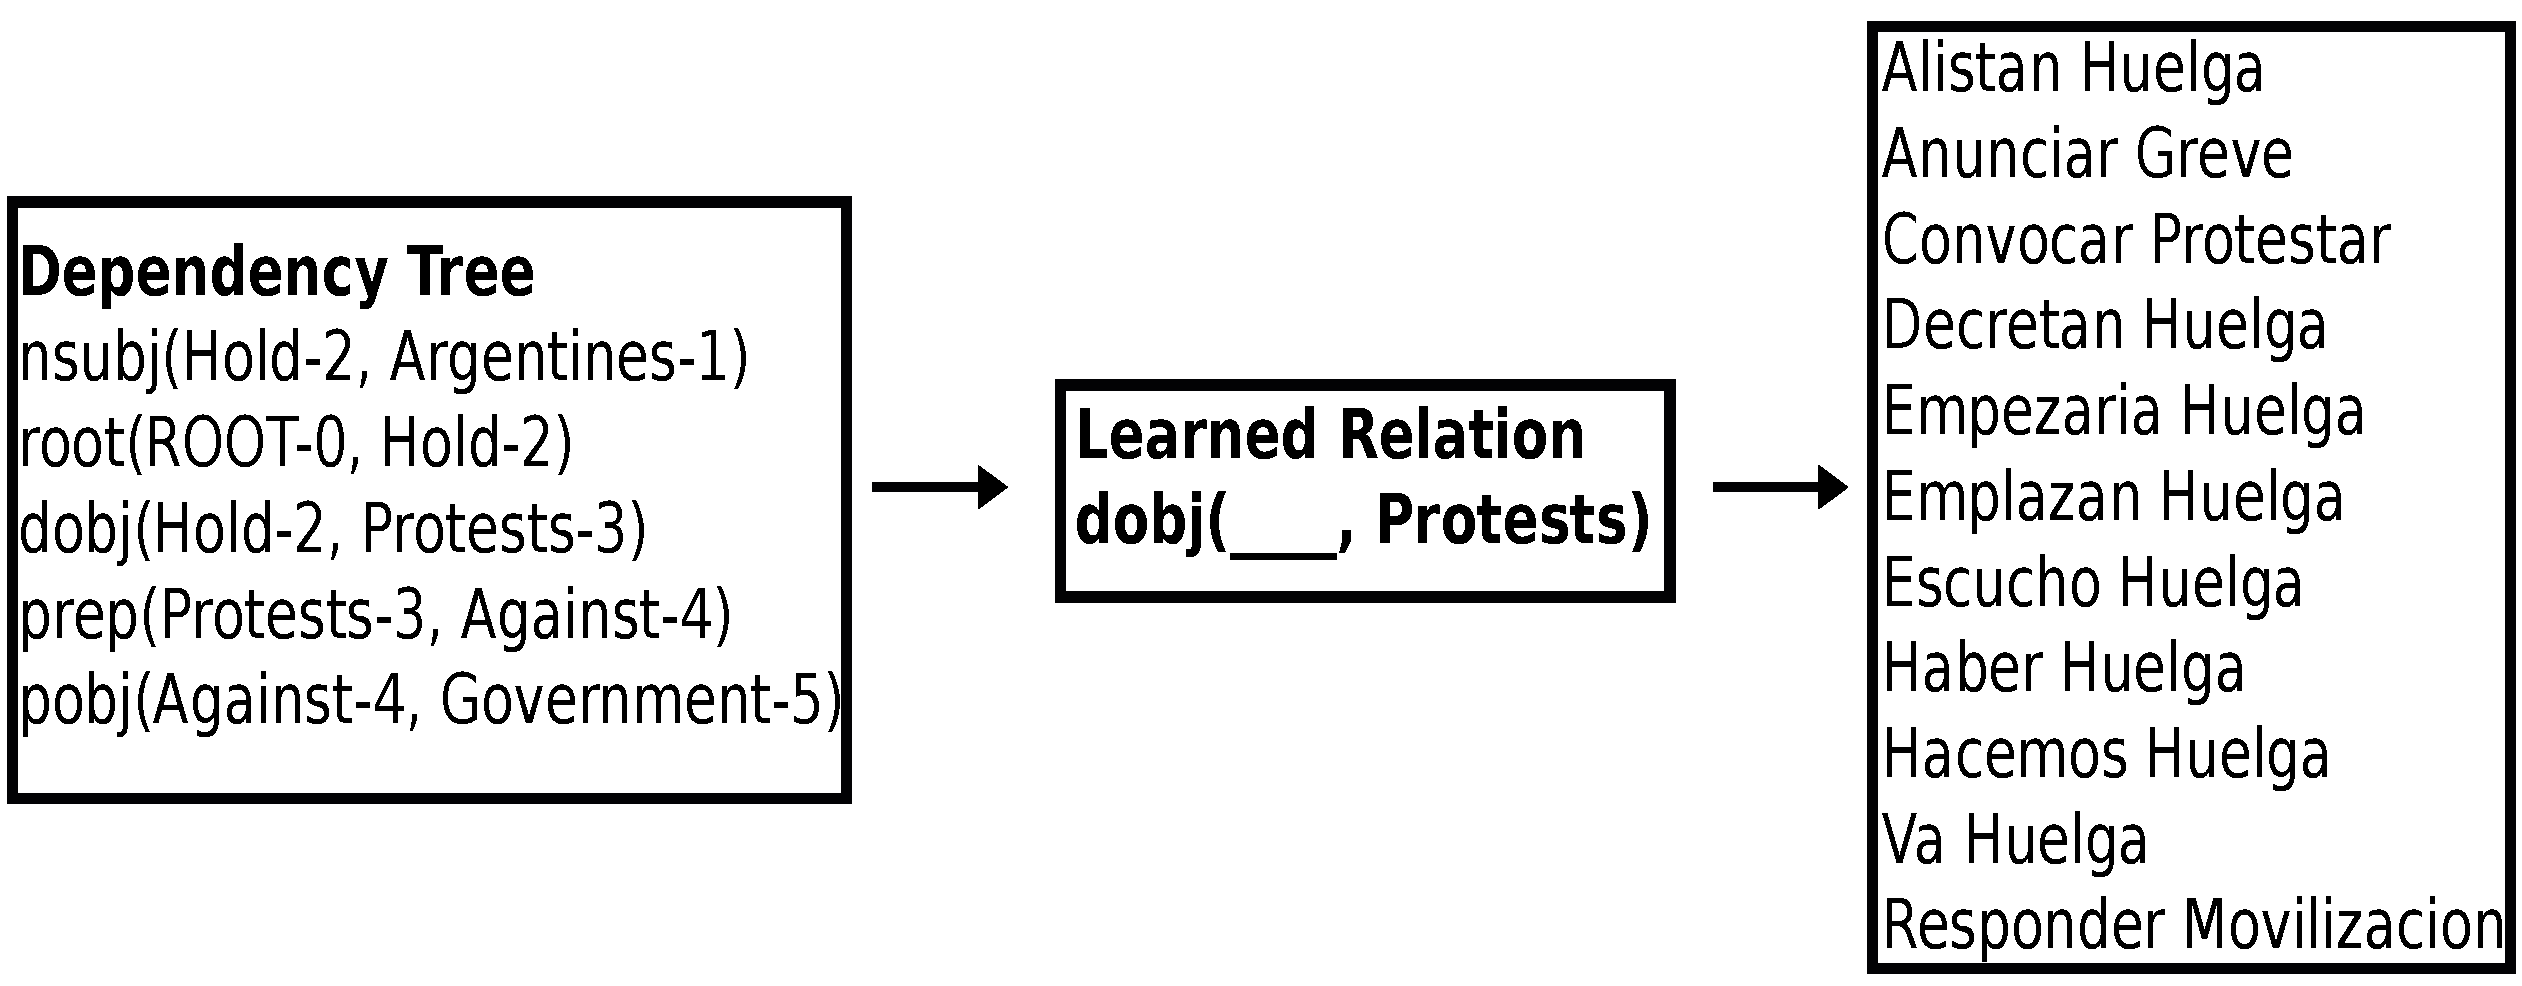
\includegraphics[width=0.5\textwidth]{figures/phraseLearning}
\vspace{-2em}
\caption{An example of phrase learning for detecting planned protests.}
\label{fig:phraselearning}
\end{figure}

\subsection{Geocoding}
\label{subsection:geocoding}
After linguistic preprocessing and suitable phrase filtering,
messages are geocoded with a
specification of the geographical focus of the text---specified as a
city, state, country tripple---that indicates the locality that the
text is about. We make use of different geocoding methodologies
for Twitter messages, for Facebook Events pages, and for news articles and blogs.
These are described below.

\subsubsection{Twitter}
For tweets, the geo-focus of the message is generated by a fairly
simple set of heuristics.  In particular, Twitter
geocoding is achieved by first considering the most reliable but least
available source, the geotag (latitude, longitude) of the tweet itself (this is available
for about 10% of our sample from Twitter). This provide an exact
geographic location that can be reverse geocoded into a place name
and used as the geo-focus. We find the nearest geo-coded point in
our extended gazetteer (using a kd-tree data structure) for this
purpose. If the tweet is not geocoded, we consider Twitter {\it places}
metadata and use place names present in these metadata fields to
geocode the place names into geographical coordinates. Finally, if
none of this is available, we consider the text fields contained in
the user profile (location, description) as well as the tweet text
itself to find mentions of relevant locations.  Additional toponym disambiguiation heuristics are used to
identify the actual referent of the mention.

\subsubsection{Facebook}
Similar methods are used to geocode event data extracted from Facebook event pages.  
Since only Facebook events that have a venue are used and since the
 venue of a Facebook event generally specifies a latitude, longitude, and physical address information, 
identifying the locatino is a fairly trivial task.  In cases where only latitude and longitude are given, 
we apply reverse-geocoding mechanisms similar to those used for Twitter.

\subsubsection{News and Blogs}
For longer articles such as news articles, the geo-focus of the message is identified using much more complex methods
To extract the protest location from news articles, we use PSL to build probabilistic models that infer the intended
location of a protest by 
weighing evidence coming from the Basis entity extractions and information in the World Gazeteer. 

The primary rules in the model encode the effect that Basis-extracted location strings that match to gazatteer 
aliases are indicators of the article's location, whether they be country, state, or city aliases. 
Each of these implications is conjuncted with an prior for ambiguous, overloaded aliases that is 
proportional to the population of the gazetteer location. For example, if the string ``Los Angeles'' appears in the article, 
it could refer to either Los Angeles, California, or Los \'{A}ngeles in Argentina or Chile. Given no other information,
our model would infer a higher truth value for the article referring to Los Angeles, California, because it 
has a much higher population than the other options. 
\begin{flalign*}
    ENTITY&(L, location) \softand REFERSTO(L, locID) &\\
                        &\rightarrow PSLLOCATION(Article, locID) &
\end{flalign*}

\vspace{-1em}
\begin{flalign*}
    ENTITY&(C, location) \softand IsCountry(C) &\\
                        &\rightarrow ArticleCountry(Article, C) &
\end{flalign*}

\vspace{-1em}
\begin{flalign*}
    ENTITY&(S, location) \softand IsState(S)&\\
                            &\rightarrow ArticleState(Article, S)&
\end{flalign*}

\noindent
(Note that the above are not deterministic rules; e.g., they do not use the logical conjunction $\wedge$ but rather the
Lukasiewicz t-norm based relaxation $\softand$. Further, these rules do not fire deterministically but are instead
simultaneously solved for satisfying assignments as described in Section~\ref{section:PSL}.)

The secondary rules, which are given half the weight of the primary rules, perform the same mapping of extracted strings 
to gazetteer aliases, but for extracted persons and organizations. Strings describing persons and 
organizations often include location clues (e.g., ``mayor of Buenos Aires''), but intuition suggests 
the correlation between the article's location and these clues may be lower than with location strings. 
\begin{flalign*}
    ENTITY&(O, organization) \softand REFERSTO(O, locID)&\\
                            &\rightarrow PSLLOCATION(Article, locID) &
\end{flalign*}

\vspace{-1em}
\begin{flalign*}
    ENTITY&(O, organization) \softand IsCountry(O)&\\
        &\rightarrow ArticleCountry(Article, O)&
\end{flalign*}

\vspace{-1em}
\begin{flalign*}
    ENTITY&(O, organization) \softand IsState(O)&\\
          &\rightarrow ArticleState(Article, O) &
\end{flalign*}
Finally, the model includes rules and constraints to require consistency between the different levels of geolocation, 
making the model place higher probability on states with its city contained in its state, which is 
contained in its country. As a post-processing step, we enforce this consistency explicitly by using the 
inferred city and its enclosing state and country, but adding these rules into the model makes the 
probabilistic inference prefer consistent predictions, enabling it to combine evidence at all levels.
As an example of how PSL aids in location identification, the example from Fig.~\ref{pp_example}
is revisited in Fig.~\ref{fig:psl_example}. 
\begin{flalign*}
    PSLLOCATION&(Article, locID) \softand Country(locID, C)&\\
               &\rightarrow ArticleCountry(Article, C)&
\end{flalign*}

\vspace{-1em}
\begin{flalign*}
    PSLLOCATION&(Article, locID) \softand Admin1(locID, S)&\\
               &\rightarrow ArticleState(Article, S)&
\end{flalign*}

\begin{figure*}
    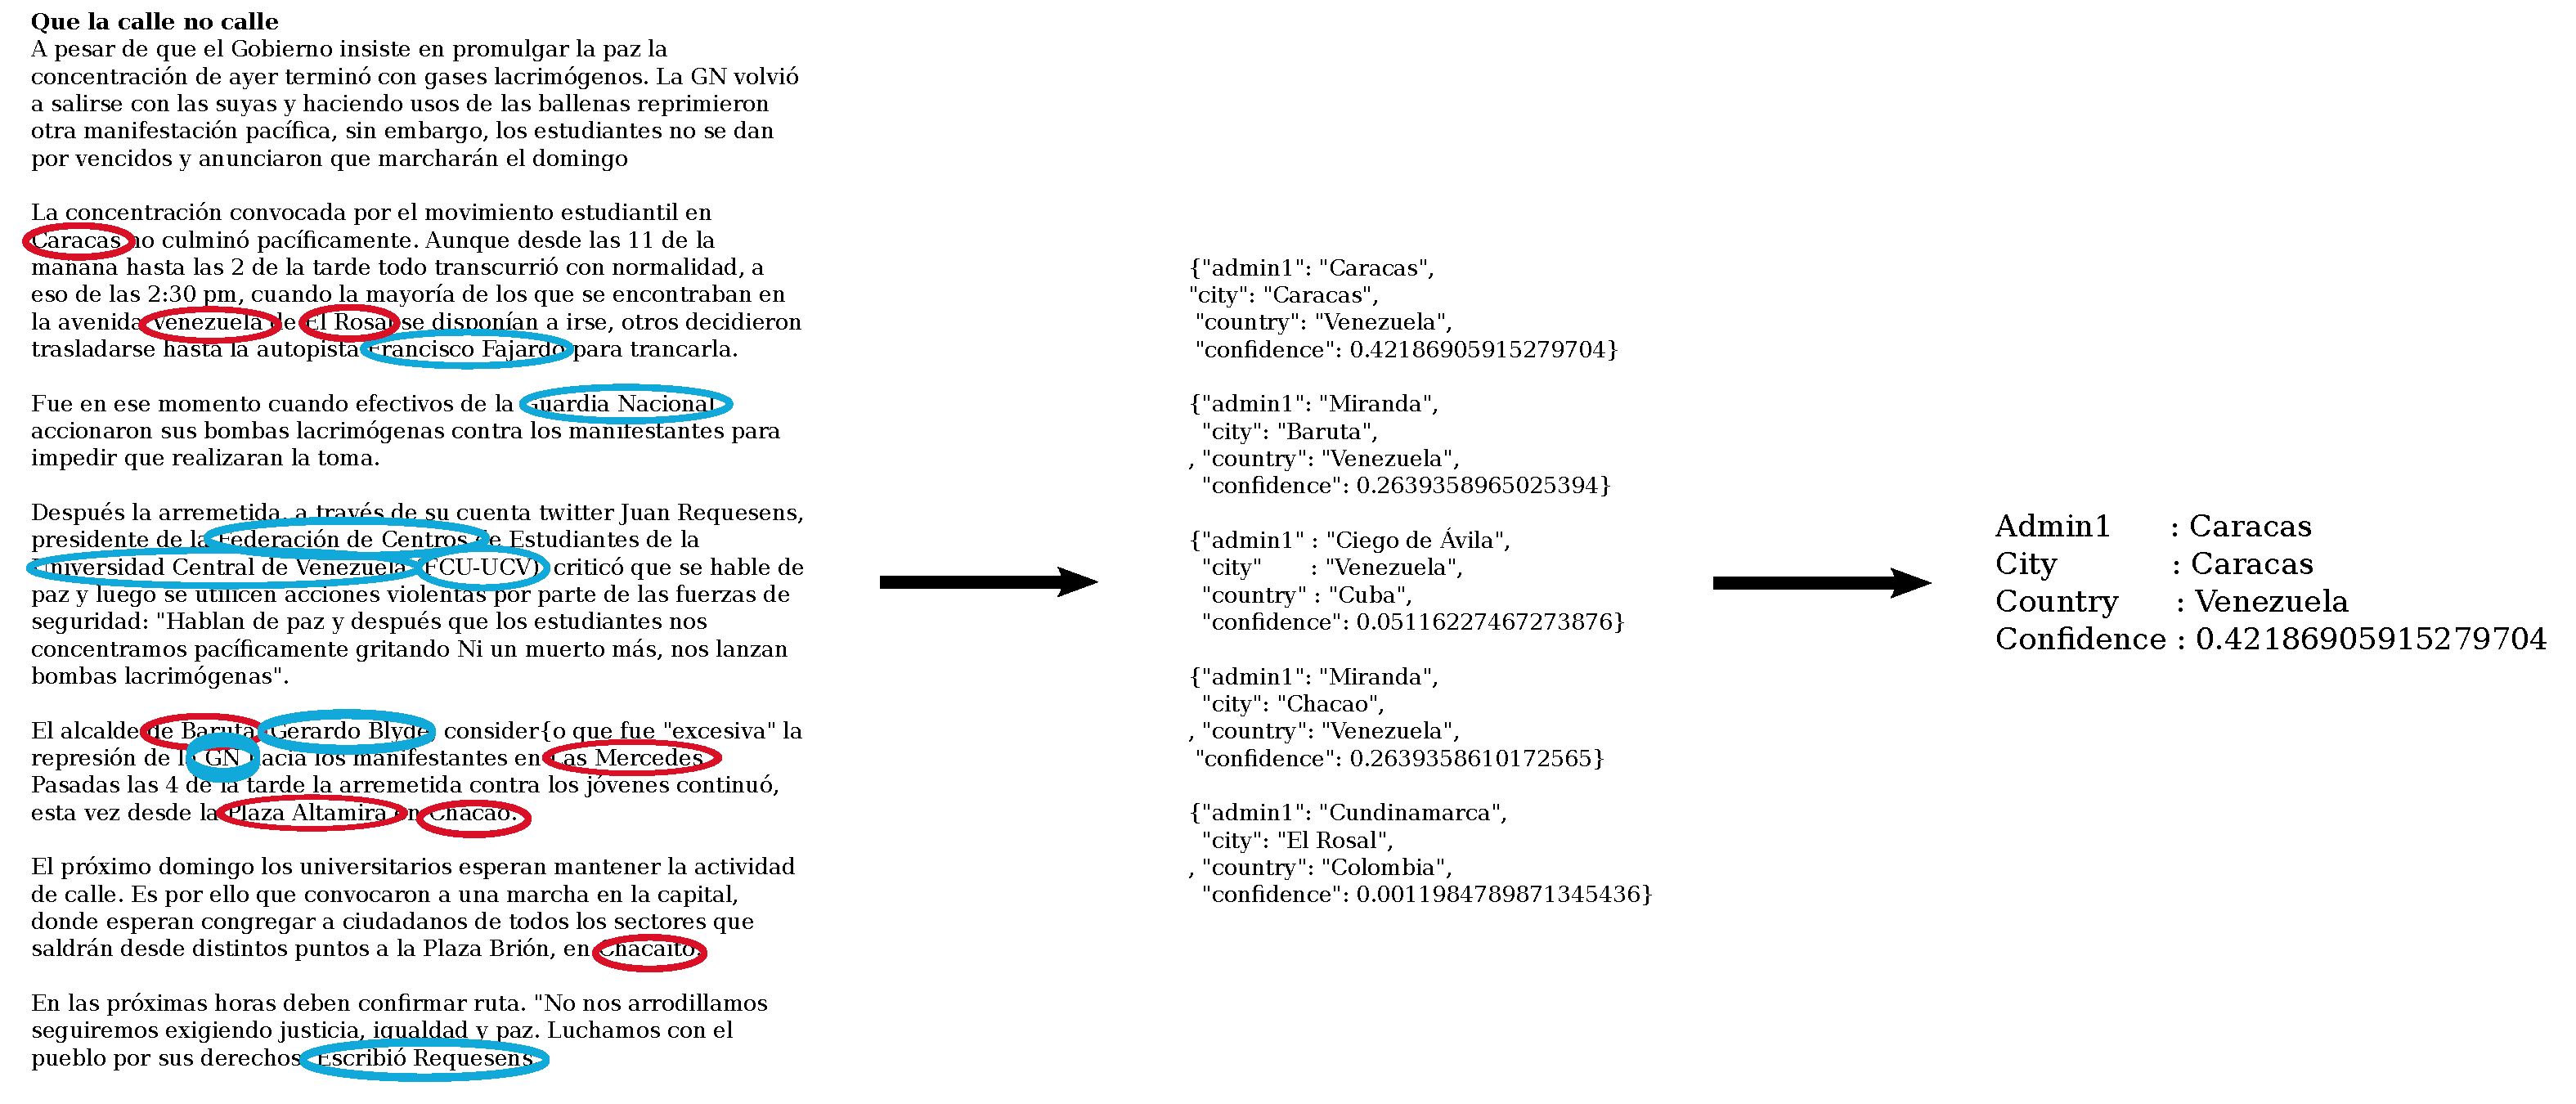
\includegraphics[width=\textwidth]{psl_pipeline2}
    \vspace{-2em}
    \caption{An example of location inference using PSL. Red circles denote named entities identified as locations and blue denotes other types of entities. The 
article describes students planning a march on Sunday.
It identifies multiple locations, e.g., Chacao, El Roso, and the Francisco Fajardo highway where protests have been happening.
There is also a reference to a quote by the mayor of Baruto.
Mentions of such multiple locations are resolved using our PSL program to the intended location, here Caracas.}
    \label{fig:psl_example}
\end{figure*}

%%!TEX root = ../plannedprotest.tex

To extract the protest location from news articles, we use \emph{probabilistic soft logic} (PSL) \cite{broecheler:uai10;kimmig:probprog12} to build a model that performs robust, probabilistic inference given noisy signals. PSL takes a set of weighted, logic-like rules and converts them into a continuous probability distribution over the unknown truth values of logical facts. These truth values in PSL are relaxed into the $[0,1]$ interval. We use this mechanism to build a model that infers the semantic location of an article by weighing evidence coming from the Basis entity extractions and information in the World Gazatteer. 

The primary rules in the model encode the effect that Basis-extracted location strings that match to gazatteer aliases are indicators of the article's location, whether they be country, state, or city aliases. Each of these implications is conjuncted with an prior for ambiguous, overloaded aliases that is proportional to the population of the gazetteer location. For example, if the string ``Los Angeles'' appears in the article, it could refer to either Los Angeles, California, or Los \'{A}ngeles in Argentina or Chile. Given no other information, our model would infer a higher truth value for the article referring to Los Angeles, California, because it has a much higher population than the other options. 

The secondary rules, which are given half the weight of the primary rules, perform the same mapping of extracted strings to gazetteer aliases, but for extracted persons and organizations. Strings describing persons and organizations often include location clues (e.g., ``mayor of Buenos Aires''), but intuition suggests the correlation between the article's location and these clues may be lower than with location strings. 

Finally, the model includes rules and constraints to require consistency between the different levels of geolocation, making the model place higher probability on states with its city contained in its state, which is contained in its country. As a post-processing step, we enforce this consistency explicitly by using the inferred city and its enclosing state and country, but adding these rules into the model makes the probabilistic inference prefer consistent predictions, enabling it to combine evidence at all levels.
\iffalse Most news articles and blog posts mention multiple locations, e.g.,
the location of reporting, the location of the incident, and locations corresponding
to the hometown of the newspaper. We developed a probabilistic reasoning
engine using probabilistic soft logic (PSL)
to infer the most likely city, state and country which is the main geographic focus the article.The PSL geocoder combines various types of evidence, such as named entities
such as locations, persons, and organizations identified by RLP, as
well as common names and aliases and populations of known
locations. These diverse types of evidence are used in weighted rules
that prioritize their influence on the PSL model's location
prediction. For example, extracted location tokens are strong
indicators of the content location of an article, while organization
and person names containing location names are weaker but still
informative signals; the rules corresponding to these evidence types
are weighted accordingly.

The methodology is similar to {\em Web-a-where: Geo-Tagging Web Content}.
\fi 

%\begin{figure}
%    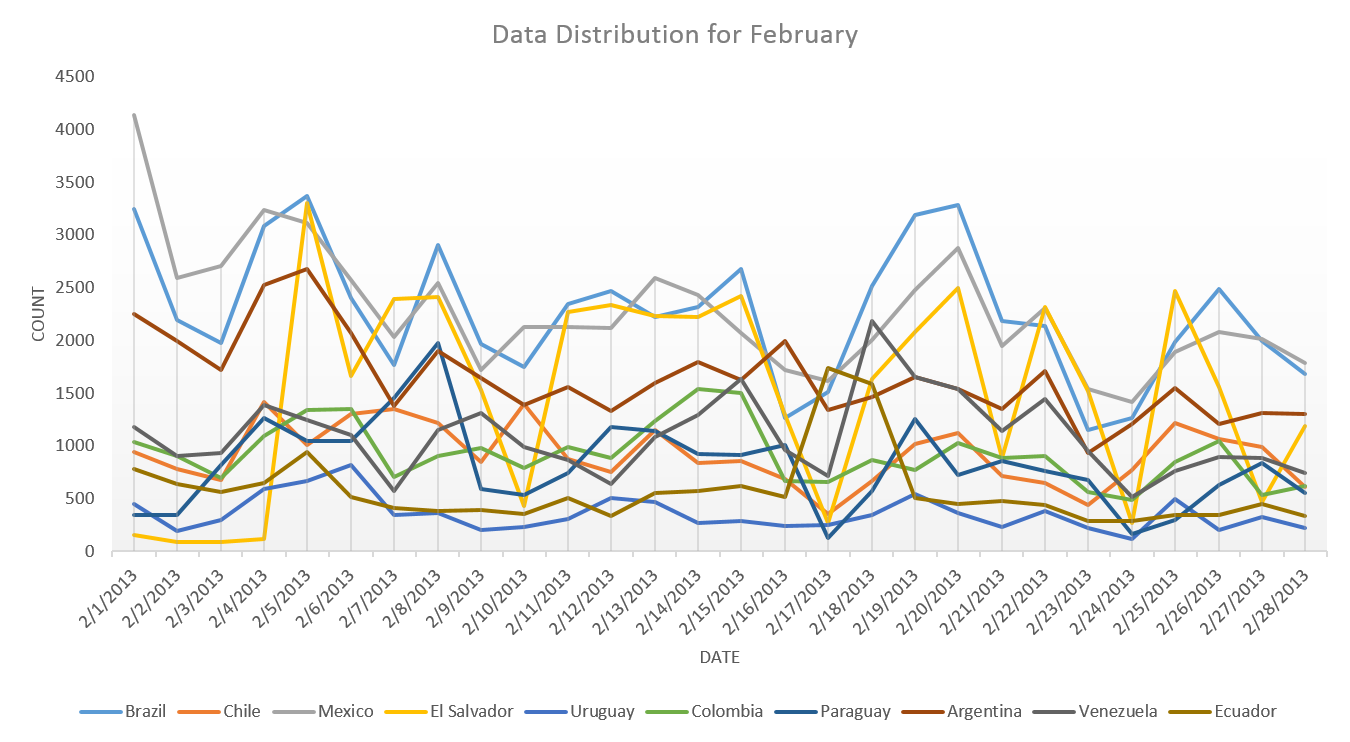
\includegraphics[width=0.5\textwidth]{rssdistribution}
%    \caption{Rate of Arrival of News/Blogs}
%    \label{fig:rssdistribution}
%\end{figure}
%
\subsection{Warning Generation}
After being subject to the preprocessing steps, above, all documents
that are identified as containing a key phrase are further filtered by
searching for the presence a future date in the passage containing the
key phrase and for the existence of an identified geographical focus for the text.
Documents that meet all these critera are used as the basis for a warning about a
planned civil unrest event (Twitter postings are only used as the basis for a warning
if the tweet is re-tweeted at least five times). 
A warning is generated for the date indicated by the future date
expression and the location which is the geographical focus of the
document.  
In the case of Facebook, an event page is considered to be good evidence for an alert if
there are more attendees for the event than rejects.  The date and
location are read off from the event page directly.
